%!TEX root = ../../main.tex
%----------------------------------------------------------------------------
\chapter{Financial Aspects}\label{chap:financial_aspects_chapter}
%----------------------------------------------------------------------------
The up and coming start-up "Super Smart SDU Robotics Graduates A/S" is planing to expand into a new business area. For this, the idea is to set up a a fully automated LEGO Bricks sorting and packaging line. People will be able to send in their old LEGO bricks and get paid by weight. The income comes from customers ordering very specific combinations of LEGO bricks at a far lower price point then ordering them directly at LEGO or at a toy store. \\
	\begin{figure}[H]
        \centering
        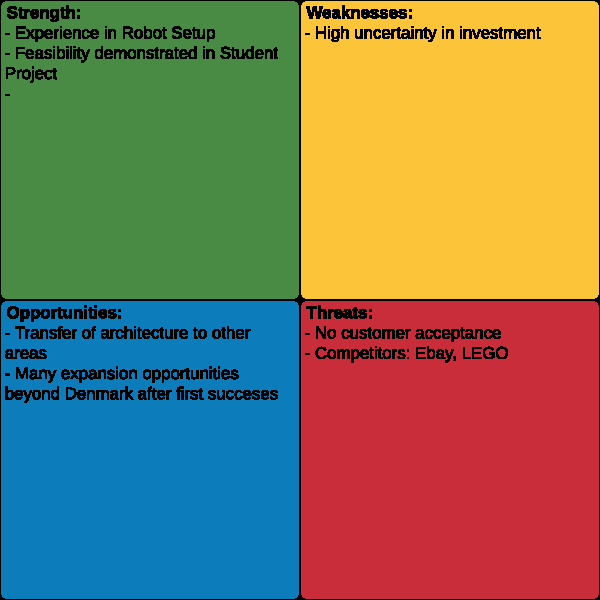
\includegraphics[width=0.6\textwidth]{swot}
        \caption{SWOT-Analysis}
        \label{fig:swot}
    \end{figure}
The SWOT-Analysis was done within the magement and an external consultant as seen in figure \ref{fig:swot}
\begin{table}[]
\centering
\begin{tabular}{llll}
\textbf{Name}          & \textbf{Type} & \textbf{Cash Flow} & \textbf{Anual increase} \\
Kuka Robot             & one-time      & -250.000           &                         \\
Frobit Robot           & one-time      & -100.000           &                         \\
Set-up labor cost      & one-time      & -300.000           &                         \\
Maintenance - Hardware & anual         & -10.000            & 4\%                     \\
Maintenance - Labor    & anual         & -78.000            & 5\%                     \\
Income                 & anual         & 250.000            & 10\%                   
\end{tabular}
\caption{Market Research}
\label{tab:market_research}
\end{table}
A careful organized market research has been done to analyse the feasibility of said proposal. This results of the market research, figure \ref{tab:market_research}, shows both the potential annual income as well as estimated investment cost.
The labour cost are based on an engineering salary of DKK 1.500 per hour. For the set-up, 200 engineer-hours are budgeted and for maintenance one hour per week. Salary is set to increase by 5\% and the maintenance annually by 4\% . These values are chosen very conservative (above the raw material price index for maintenance material and above the average salary increase over the past five years) to allow for fluctuation and uncertainties. \\ The income growth over the first five years is set to constant 10 \% even though a steeper increase is expected after the first market penetration.\\
    \begin{figure}[h]
        \centering
        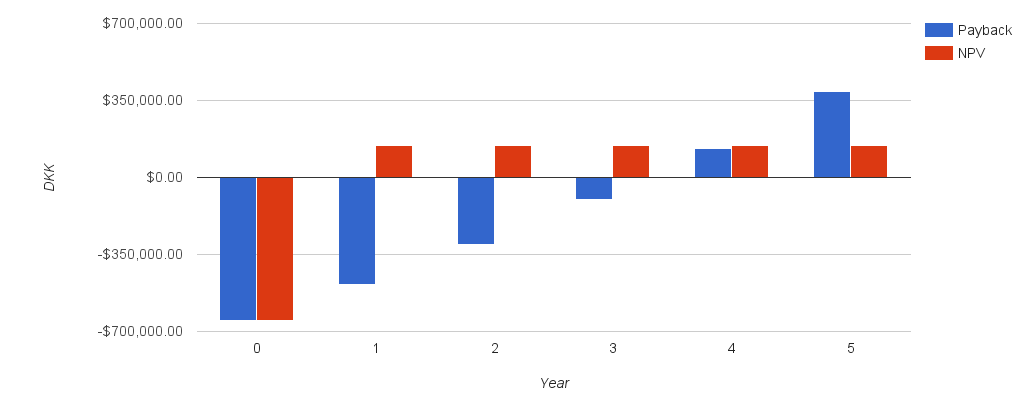
\includegraphics[width=1.0\textwidth]{figs/pb_npv}
        \caption{Payback Method and Net Present Value}
        \label{fig:payback_npv}
    \end{figure}

Given these assumptions the pay-back method \ref{fig:payback_npv}(blue) , the internal rate of return method(IRR) and the net-present value(NPV) \ref{fig:payback_npv}(red) are calculated to determine the feasibility of this investment.
The pay-back method shows a profit of DKK 390.000 after five years. The investment was judged as having a medium risk, but for calculating the NPV the required rate of return of investment has been set to 12\% to be conservative. With this the NPV of this investment after considering five years with the given assumptions would be DKK 80.000 and thus the investment is seen as favourable. The IRR is 16.47\% , this far exceeds simply investing in bonds, or paying back current bank loans, of which the highest is DKK 2.000.000 at 7\%.
All methods suggest this investment is profitable and the financial department gives the project the go-ahead.

%%% Local Variables:
%%% mode: latex
%%% TeX-master: "main"
%%% End: